\section{Design}
\label{section:design}

In this section we describe the design of our classes and algorithms based on
the requirements established in \ref{section:requirements}.

\subsection{How to Run the Subsetter}

The success of the NetCDF Operators and similar tools demonstrate the need for
user-ready applications for the analysis of their data while the success of
tools such as CDAT validate the need for a scriptable interface and customization of
basic and advanced operators.  We plan to provide both the scriptable
interface as well as a set of predefined tools.

The subsetter is the first in a series of planned parallel command-line tools
based on unstructured grids and the PGAS programming model.  It takes
arguments specifying specific variables (-v) or dimension ranges (-d) to
extract, or at a higher level a latitude and longitude bounding box (-b).  In
this way it is most akin to the NetCDF Operators' "kitchen sink" application.
Example usage looks like: \begin{itemize} \item mpiexec -np 128 subsetter -b
20,-20,160,90 -v vorticity january.nc february.nc MJO\_vorticity\_janfeb.nc
\item mpiexec -np 64 subsetter -b 90,0,180,-180 -d levels,1,5 geopotential.nc
\end{itemize}

\subsection{Dataset Abstraction}

The subsetter minimally supports two forms of input file aggregation, either
across a specified dimension e.g. time or by taking the union of all input
files such that duplicate dimensions and variables within later files are
ignored.  These forms of aggregation are modeled after what is available when
using NetCDF Markup Language.\cite{NcML} NcML input is not directly supported
at this time but is planned for a future release. 

\subsection{Parallel IO Abstraction}

IO operations are hidden behind abstract base classes.  Any IO library can be
supported.  This is similar to how the Java NetCDF library works
\cite{JavaNetCDF}.  Further, differing IO strategies using the same IO library
can also be developed behind the same API.  The use of Parallel NetCDF was
selected because of the ubiquity of the NetCDF libraries and data format in
climate applications.

\subsection{The Global Arrays Library}

The partitioned global address space (PGAS) programming model assumes a global
address space which is partitioned such that each process is associated with a
local portion of the space.  One-sided communication allows a process to
access another process's address space without any explicit participation by
the latter process.  Such communication can reduce synchronization, reduce
data movement, and can simplify programming.  The Global Arrays (GA) library
supports both models.

The subsetter was built using the GA library for the wealth of features it
provides which are tailored to our problem domain.  GA provides a distributed
dense multidimensional array programming abstraction and the data we will be
operating over is stored as dense arrays within NetCDF files.  It should be
noted that dense distributed arrays would also work well for regularly gridded
data.  However, due to the use of unstructured grid data, the algorithm for
subsetting the data will look quite different than for the structured case.
Recall that for unstructured grids, logically adjacent cells are not
necessarily adjacent in memory.  In order to evenly distribute a subset, a
single process will need to send a varying amount of data to any number of
other processes.  Certainly a collective operation could be considered, but GA
provides the necessary functionality without needing any explicit cooperation
from any other process.  Any given process will simply put the section of the
subset into the remote process's memory.

There are certain GA one-sided operations which are tailored for use on
one-dimensional arrays which are prevalent within our data.  These operations
include \verb=GA_Patch_enum=, \verb=GA_Scan_add=, \verb=GA_Scan_copy=,
\verb=GA_Pack=, and \verb=GA_Unpack=.  Those operations have been demonstrated
in the computation of sparse matrix multiplication\cite{GA} but are equally
useful in the manipulation of unstructured grids.  The remaining GA operations
are N-dimensional and include \verb=NGA_Scatter=, \verb=NGA_Gather=,
\verb=GA_Put=.  Those operations are useful for redistributing the subset
data.

\subsection{The Algorithms}

The one-sided communication and PGAS model supported by GA allowed us to
develop some novel algorithms for the manipulation of unstructured grids.  In
this section we diagram and describe the algorithms we developed.  The vast
majority of functionality within the subsetter is provided by either PnetCDF
or GA.  GA allocates and evenly distributes the arrays which are then filled
with data by PnetCDF.  GA operations are then used to prepare the data for
packing at which point a custom n-dimensional packing routine is used.  The
packed, evenly-distributed data is then written back to disk using PnetCDF.
Of these algorithms, the novel ones include reindexing the masks, reindexing
the topology variables, and the n-dimensional pack routine.

Each dimension of the data has two arrays associated with it, a bitmask and an
integer array representing the new indices of the dimension in case of a
subset.  For instance, if any of the bits are turned off, the corresponding
indices of the index array will have negative values.  The remaining values of
the index array will increase monotonically, skipping the negative or masked
indices.  The bitmasks are generated based on a rectangular latitude and
longitude region specified on the command-line, or by specifying one or more
indices of a dimension to select.  Although a rectangular region is currently
used for simplicity, once translated the bitmasks allow for arbitrary subsets
to be defined.  These bitmasks are then used to evenly distribute the
resultant subset across all processes.  Note that these bitmask and associated
index arrays are one-dimensional and distributed.

\subsubsection{Partial Sum}

\begin{figure}[!t]
\center
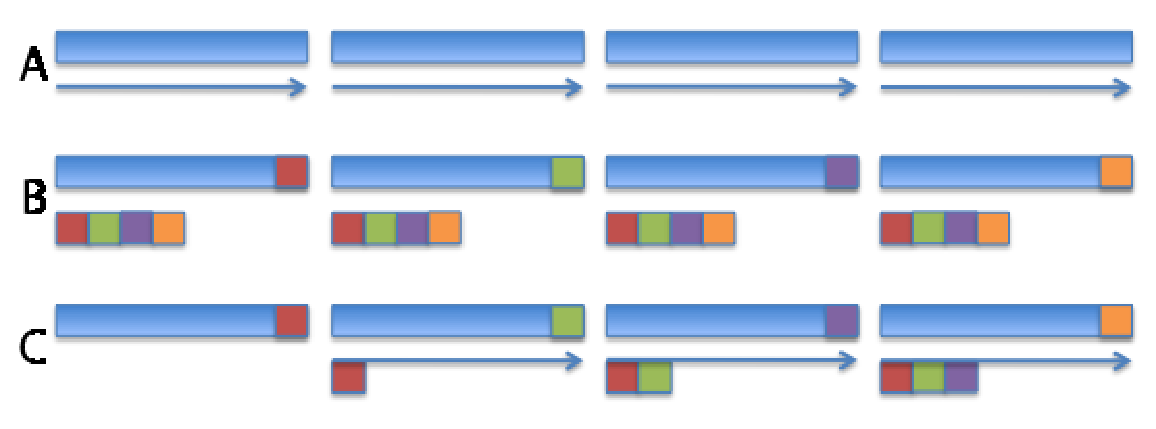
\includegraphics[width=3.5in]{images/partialsum_label}
\caption{Distributed partial sum on a 1-D array}
\label{fig:partialsum}
\end{figure}

A partial sum of the index array associated with each dimension is useful for
later determining where subset data is to be placed.  That feature will be
explained in more detail in \ref{section:alg_pack}.  The partial sum operation
here is semantically similar to the one found in the C++ STL\cite{CXXSTL}.  It
computes a series of sums over an array from the first element through the
\emph{i}th element and stores the result of each such sum in the \emph{i}th
element of a destination array.

The partial sum is computed by first performing partial sums of each local
portion of the source array.  This operation is represented by Figure
\ref{fig:partialsum}A.  The last value of each local sum is then collectively
distributed to each process as seen in Figure \ref{fig:partialsum}B.  Figure
\ref{fig:partialsum}C is the last step where each local portion adds the last
values of each process's sum which come before.

\subsubsection{Reindexing of Dimension Index}

\begin{figure}[!t]
\center
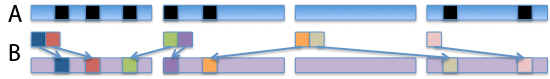
\includegraphics[width=3.5in]{images/unpack_label}
\caption{Reindexing of a Dimension Index}
\label{fig:unpack}
\end{figure}

Creating the index array associated with a mask requires three specific GA
operations, \verb=GA_Fill=, \verb=GA_Patch_enum= and \verb=GA_Unpack=.  The
mask array is represented in Figure \ref{fig:unpack}A.  \verb=GA_Fill= fills
the index array, the bottom array in Figure \ref{fig:unpack}B,  with a value
of $-1$.  A second array is created after each process counts how many masked
bits are present and collectively sums to get the size of the array to create.
\verb=GA_Patch_enum= enumerates the values in the second array starting from
zero with an increment of 1.  The enumerated array is shown in Figure
\ref{fig:unpack}B.  \verb=GA_Unpack= expands the enumerated array values into
the filled array based on the associated mask array, seen as Figure
\ref{fig:unpack}B.

\subsubsection{Reindexing of Topology Variables}

\begin{figure}[!t]
\center
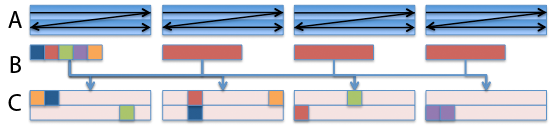
\includegraphics[width=3.5in]{images/reindex_label}
\caption{Reindexing of Topology Variables}
\label{fig:reindex}
\end{figure}

Recall that the topology variables are those which map from one index to
one or more other indices such as from a cell index to each of its corner
indices.  A typical subset operation reduces the number of cells, corners, and
edges within the grid, so it is important to maintain the integrity of these
mapping arrays such that they map to real indices.

The reindexing of the topology variables relies on the recalculated index
array of the associated domain.  For example, when reindexing the mapping from
edges to corners, the recalculated corners index array is required.  The
mapping values represent indices into the recalculated index array.  The
mapping arrays are iterated over to gather the required indices for the
subsequent GA routine \verb=NGA_Gather= to query, represented in Figure
\ref{fig:reindex}A.  The \verb=NGA_Gather= routine gathers array elements from
a global array into a local array.  In this each process gathers the new
values for the mapping from the index array (Figure \ref{fig:reindex}B) and
then appropriately replaces the old mapping values in Figure
\ref{fig:reindex}C.

\subsubsection{N-Dimensional Pack}
\label{section:alg_pack}

\begin{figure}[!t]
\center
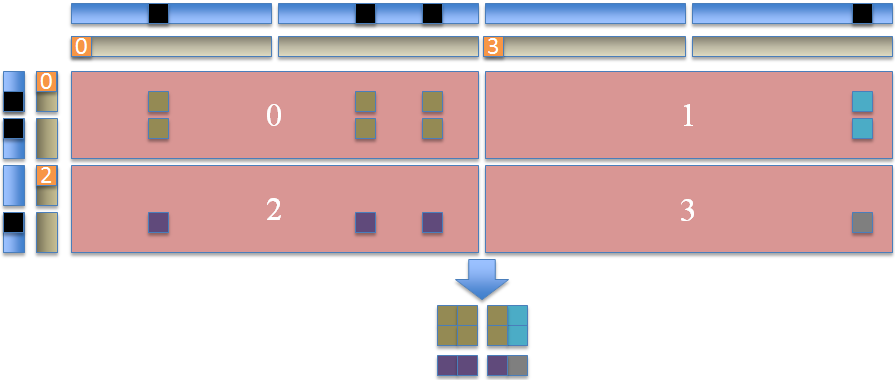
\includegraphics[width=3.5in]{images/pack}
\caption{Pack}
\label{fig:pack}
\end{figure}

The goal of the pack routine is to start with an evenly distributed source
array, subset it, and evenly distribute the subset.  The subset is specified
using mask arrays, one for each dimension of the source array.  The problem
lies with where to put the data once each process computes its portion of the
subset; each process would need to know a priori the size of the subsets that
logically come before their own computed portion and \verb=NGA_Put()= their
data after then.

The partial sum of the mask array is a convenient solution to this problem.
Each process owns a portion of the source array in terms of the global address
space of the array.  For each dimension, the value in the corresponding
partial sum array at the index represented by the lowest index owned by each
local portion describes where to put the subset data.

Figure \ref{fig:pack} should clarify this.  In the figure, the blue arrays
represent both the mask arrays as well as the partial sum arrays.  The masked
bits are indicated in black.  Each of the four processes query the partial sum
arrays using \verb=NGA_Get()= at the corresponding locations indicated in
orange and the small blue arrows.  Now knowing where to put their subset data,
each process can \verb=NGA_Put()= their portions resulting in the subset
array.  Because the destination array was created using GA, it is by
definition evenly distributed.  The \verb=NGA_Get()= and \verb=NGA_Put()=
operations do not require explicit knowledge of where the data lives,
aleviating the burder of the programmer.
